\subsection{Ca sử dụng công khai chuyến đi}
\vspace{0.5cm}


\noindent 
\begin{tabularx}{\linewidth}{| l | X |} 
\hline 
\textbf{Mô tả} & Người dùng công khai chuyến đi để mọi người tham gia. \\
\hline 
\textbf{Luồng cơ bản} & 1. Người dùng chọn một chuyến đi muốn công khai. \newline
                        2. Hệ thống lây dữ liệu chi tiết của chuyến đi và hiển thị. \newline
                        3. Người dùng bấm "Công khai". \newline
                        4. Hệ thống kiểm tra thông tin chuyến đi. \newline
                        5. Hệ thống chuyển đổi chuyến đi sang công khai và thông báo đến các tài khoản khác. \\
             
               
\hline 
\textbf{Luồng thay thế} & Chuyến đi không đủ thông tin hệ thống sẽ thông báo lỗi chưa đủ thông tin. \\
       
\hline 
\textbf{Tiền điều kiện} & - Người dùng đang đăng nhập và phiên đăng nhập chưa kết thúc.\newline
                        - Người dùng đã tạo ít nhất một chuyến đi. \newline
                        - Chuyến đi phải là chuyến di riêng tư.\\


\hline 
\textbf{Hậu điều kiện} & - Hệ thống cập nhật quyền riêng tư của chuyến đi sang công khai. \newline
- Hệ thống hiển thị chuyến đi dưới dạng bài viết trên trang chủ để mọi người tham gia. \newline
- Hệ thống gửi thông báo đến các tài khoản khác về chuyến đi công khai. \\
                        

\hline 
\textbf{Yêu cầu phi chức năng} & Hệ thống công khai chuyến đi dưới 2s \\
\hline 
\end{tabularx}

\noindent 
\begin{tabular}{| c | c |}
    \hline
    \textbf{Biểu đồ hoạt động} & \textbf{Quan hệ} \\ 
    \hline
    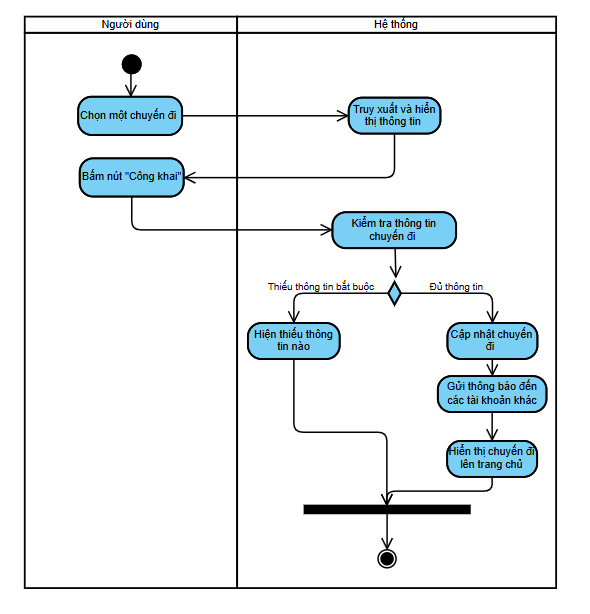
\includegraphics[width=0.5\linewidth]{figures/c3/3-3-15-ad.png} 
    & 
    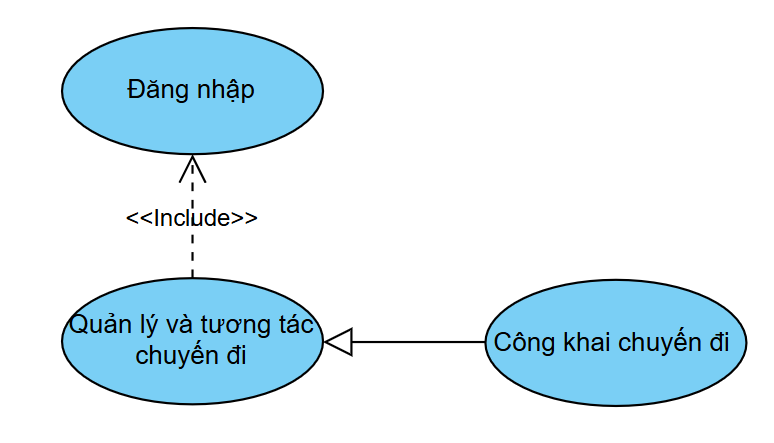
\includegraphics[width=0.45\linewidth]{figures/c3/3-3-15-rd.png} \\ 
    \hline
\end{tabular}

\vspace{0.8cm}

\begin{figure}[H]
    \centering  
    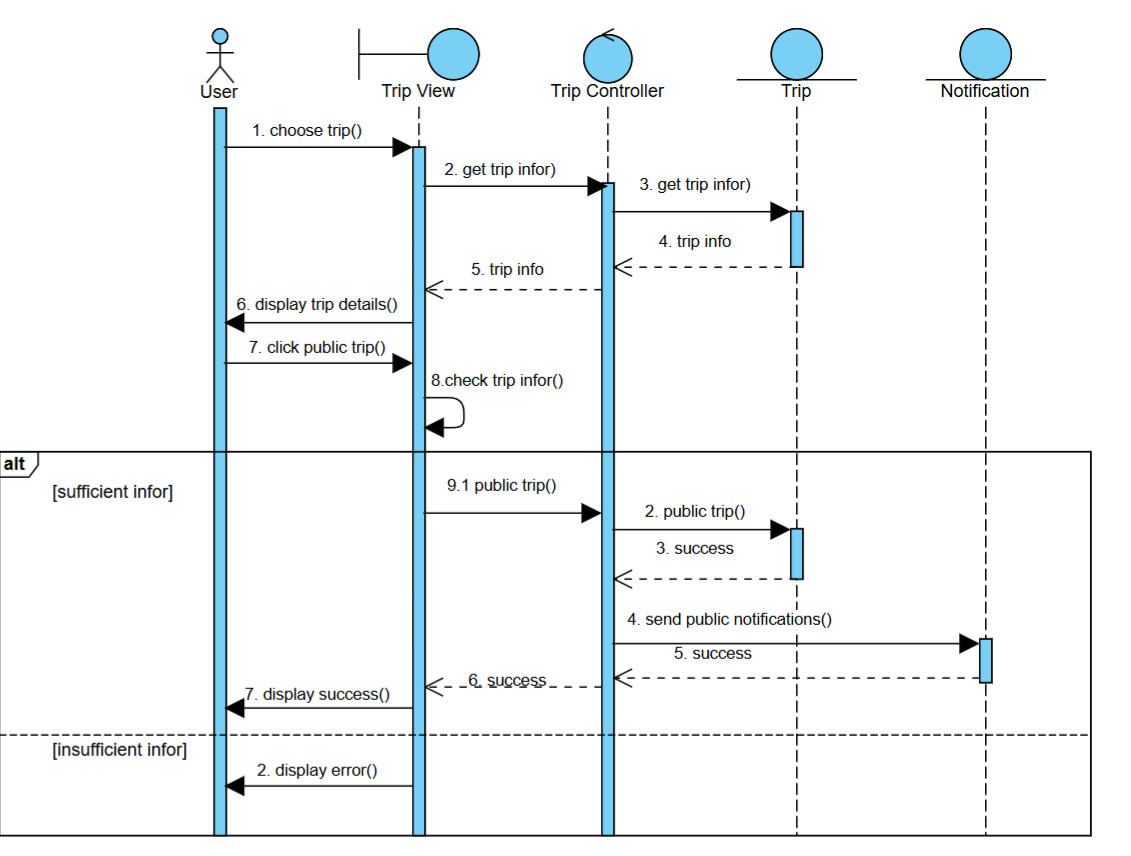
\includegraphics[width=1\textwidth]{figures/c3/3-3-15-sd.png}
    \caption{Biểu đồ tuần tự ca sử dụng công khai chuyến đi.}
    \label{fig:3-3-15-sequence-diagram}
\end{figure}